\documentclass{article}
\usepackage[utf8]{inputenc}
\usepackage{graphicx}
\graphicspath{ {./images/} }
\usepackage{geometry}
\usepackage{hyperref}
\geometry{a4paper,textheight=25cm,textwidth=15cm}

\title{Documentatie - QuizzGame (B)}
\author{Dascălu Rareș-Vasilică, Grupa A5, Anul 2}
\date{07.12.2022}

\begin{document}

\maketitle

\textbf{Abstract.} Acest document are ca scop prezentarea tehnologiilor utilizate, a arhitecturii si a detaliilor de implementare a proiectului propus QuizzGame (B)



\section*{Introducere:}

$\quad$Scopul acestui proiect este de a crea un server ce permite unui numar nelimitat de clienti sa se conecteze si sa raspunda la diferite intrebari. Serverul va retine scorurile fiecarui client si le va incrementa pentru fiecare raspuns corect. 

\section*{Motivatie:}

$\quad$Am ales acest proiect deoarece este un concept foarte asemanator cu site-ul https://kahoot.it/. Fiind un concept cunoscut, am vrut sa aflu cum functioneaza si cum se creeaza o aplicatie de acest tip. Alt motiv pentru care am ales acest proiect este ca imi place sa imi testez creativitatea in crearea jocurilor.

\section*{Tehnologii utilizate:}

$\quad$Aplicatia trebuie sa permita un numar nelimitat de clienti, de aceea protocolul folosit este de tip TCP/IP concurent, fiecare client primind la conectare un thread creat de server, in care isi va desfasura intreaga activitate. In comparatie cu protocolul UDP, acesta asigura integritatea mesajelor, precum si faptul ca mesajele ajung la destinatie in ordine cronologica.

Deoarece C/C++ este un limbaj ce se recomanda pentru proiectarea unor astfel de proiecte si ofera o varietate de functii ce ma pot ajuta sa duc la bun sfarsit acest proiect, acesta va fi utilizat pentru crearea proiectului.

Deoarece trebuie sa tinem evidenta clientilor si a intrebarilor, vom folosi o baza de date relationala, SQLite, versiunea a 3-a.

\section*{Arhitectura aplicatiei}

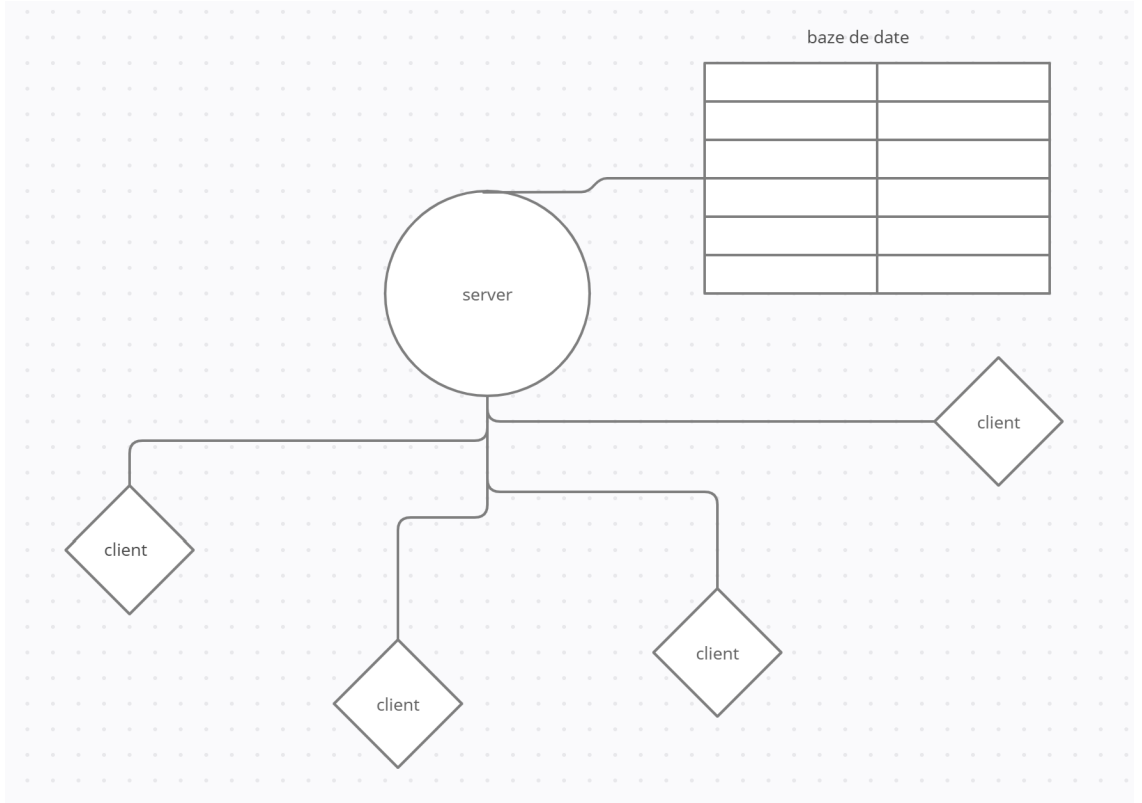
\includegraphics[scale=0.5]{1}

\section*{Detalii de implementare:}
$\quad$In prezent programul contine 4 fisiere (client.c, client.h, server.c, server.h, baza.db). 
Fisierul client.c contine clientul ce primeste de la server textul afisat de client ce specifica conectarea. Clientul trimite inapoi catre server numele si parola, serverul le verifica, si trimite inapoi un raspuns pentru a spune clientului daca a reusit sa se conecteze cu succes sau nu. 

Dupa conectare, clientul primeste de la server un meniu, oferindu-i optiunea de a iesi din joc sau de a incepe jocul. Odata ce jocul este pornit, clientul primeste de la server intrebarile si raspunsurile, avand timp cate 10 secunde pentru fiecare intrebare. Fiecare client isi calculeaza propriul scor, ce este ulterior trimis la server pentru a nominaliza un castigator.

\vspace{0.3cm}

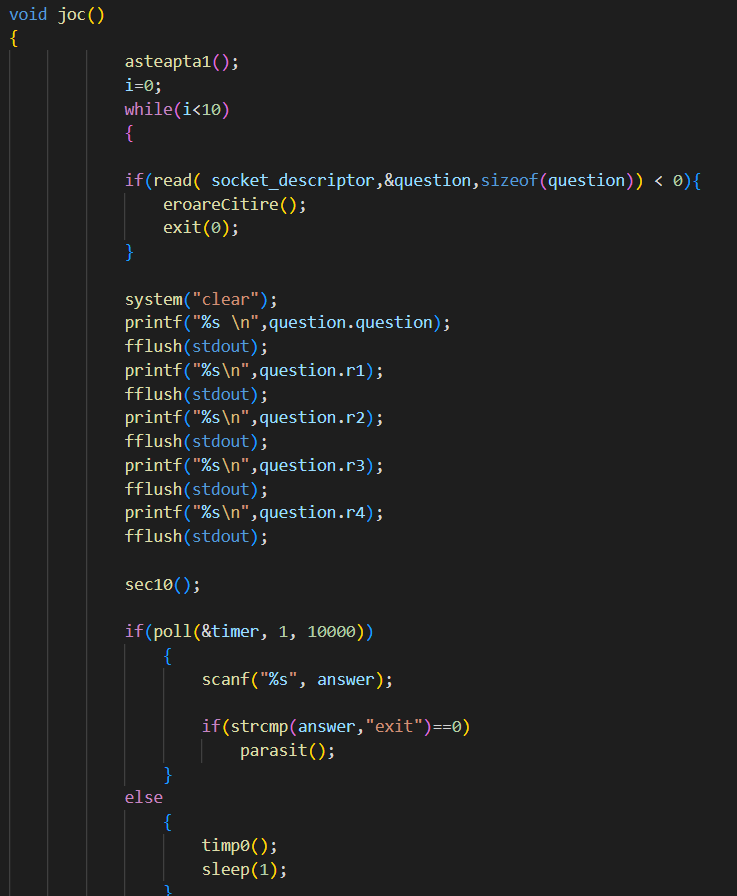
\includegraphics[scale=0.35]{client1}
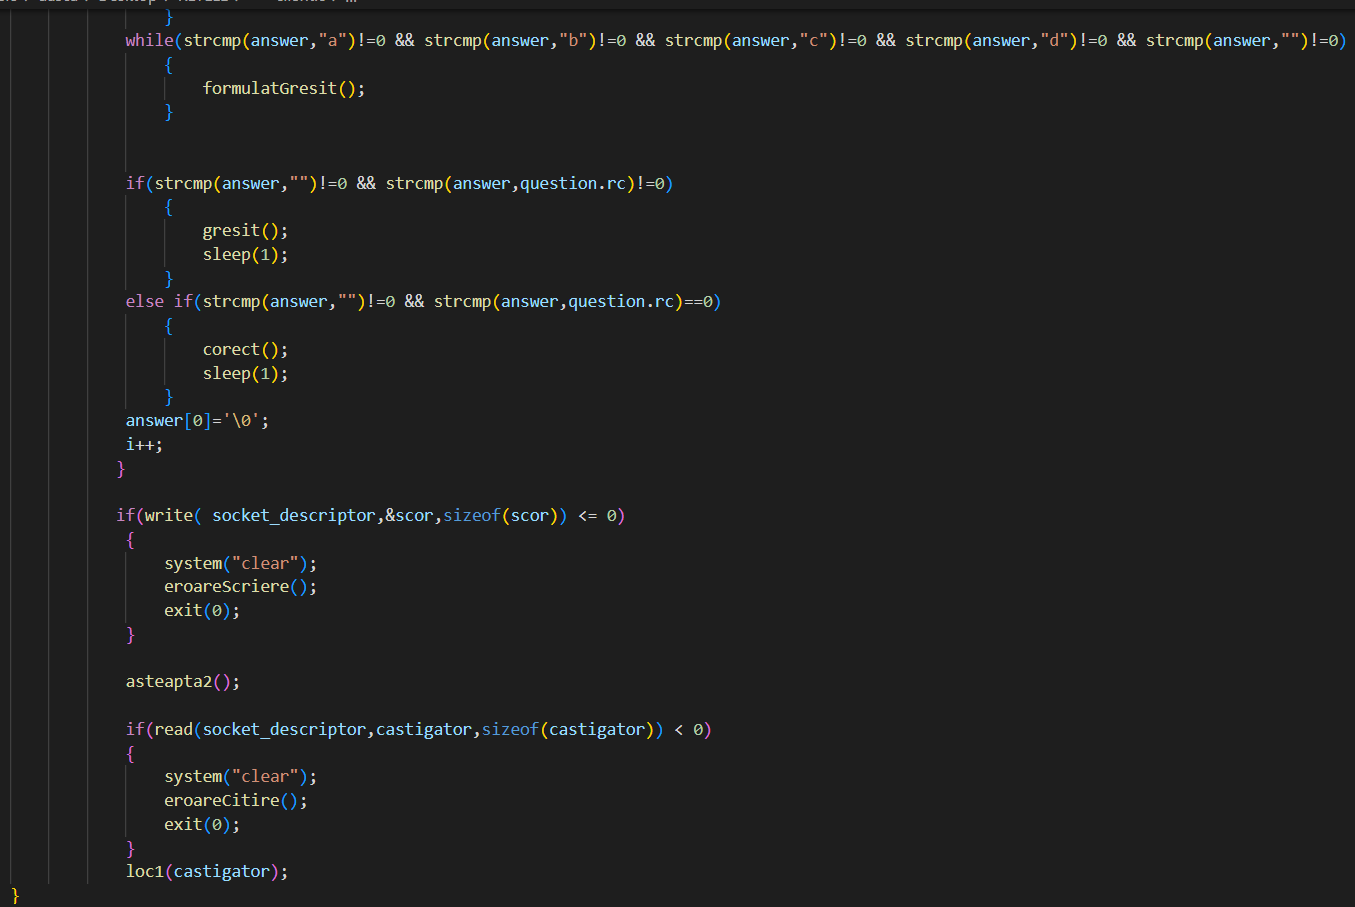
\includegraphics[scale=0.35]{client2}

\vspace{0.3cm}

Fisierul server.c contine serverul ce creaza socket-ul pentru comunicarea cu clientii. Am atasat sererul cu functia bind(), iar cu functia listen() am pus serverul sa asculte clientii ce doresc sa se conecteze. Pentru fiecare client a fost creat cate un thread pentru conectarea clientilor si executia jocului in sine pentru fiecare client in parte.

In momentul in care este apasata comanda "CTRL + C" serverul te va intreba daca doresti sa inchizi serverul pentru a nu fi inchis din greseala.

\begin{center}
\vspace{0.3cm}
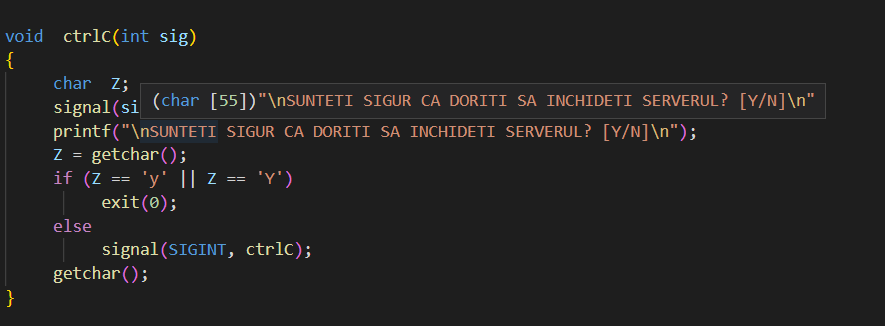
\includegraphics[scale=0.5]{server1}
\vspace{0.3cm}
\end{center}

Inainte de crearea socket-ului in server, acesta citeste intrebarile din baza de date, pentru a fi sigur ca poate incepe un joc dupa conectarea clientilor.

\begin{center}
\vspace{0.3cm}
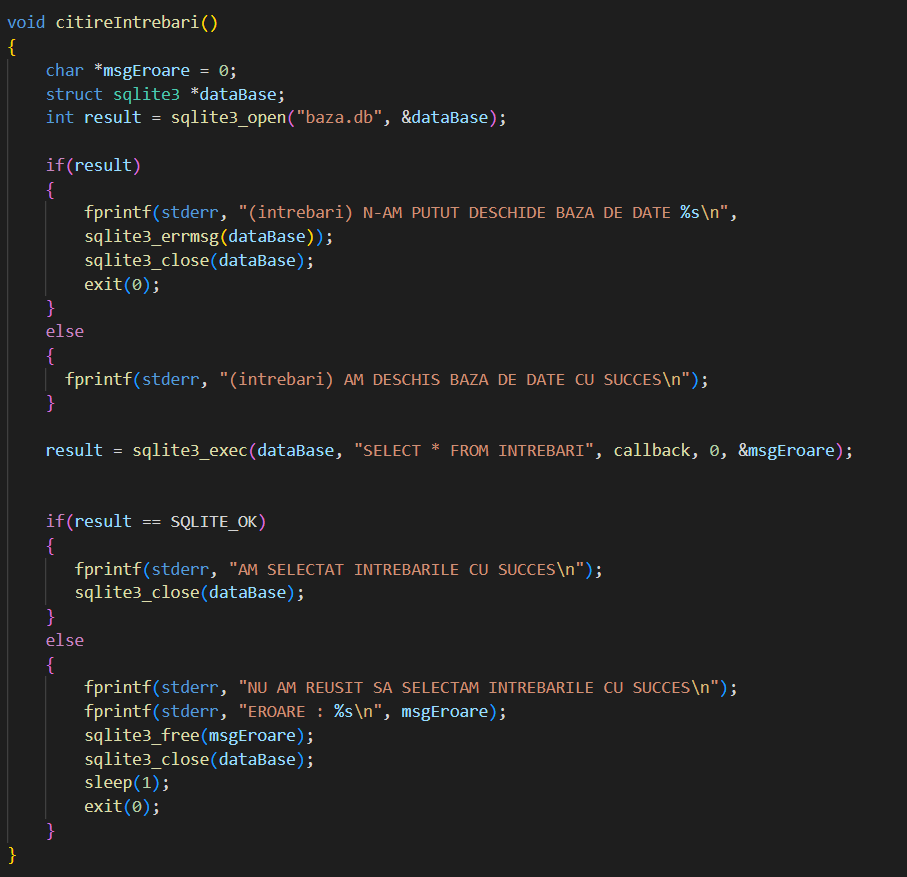
\includegraphics[scale=0.5]{server2}
\vspace{0.3cm}
\end{center}

Pentru conectarea clientului am folosit un subprogram ce verifica in baza de date existenta utilizatorului trimis de client, si corectitudinea parolei.

\begin{center}
\vspace{0.3cm}
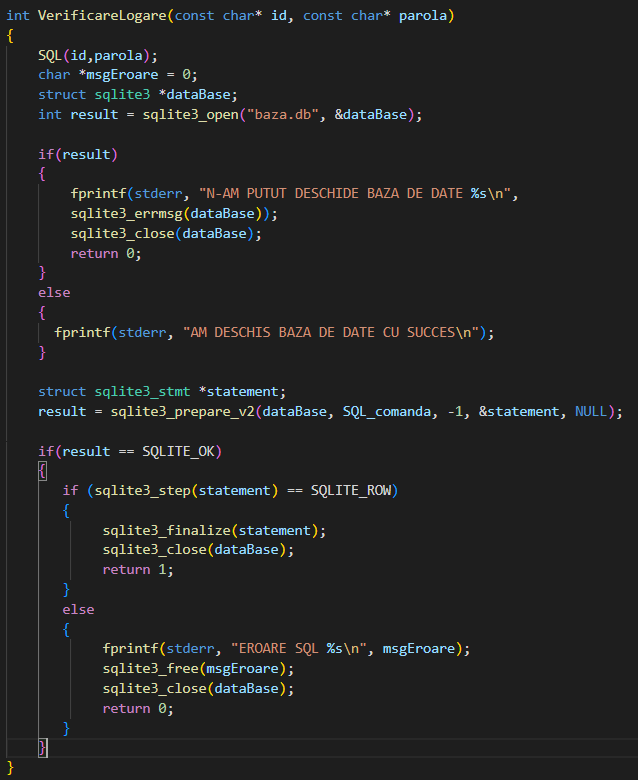
\includegraphics[scale=0.5]{server3}
\vspace{0.3cm}
\end{center}

Dupa conectarea clientului si selectarea optiunii de incepere a jocului de catre client, serverul va astepta pana toti utilizatorii conectati selecteaza inceperea jocului, in caz contrar, va astepta pana se deconecteaza cei ce nu au selectat o optiune din meniu. 

Odata ce a inceput jocul, serverul va trimite aleatoriu catre clienti 10 intrebari din lista de intrebari gasite in baza de date, incluzand si variantele de raspuns, si raspunsul corect. Dupa ce utilizatorii au terminat de raspuns la toate intrebarile, serverul va primi punctajele fiecarui client, urmand sa calculeze clientul cu cel mai mare punctaj, si ii va trimite numele castigatorului fiecarui client in parte.

\vspace{0.3cm}

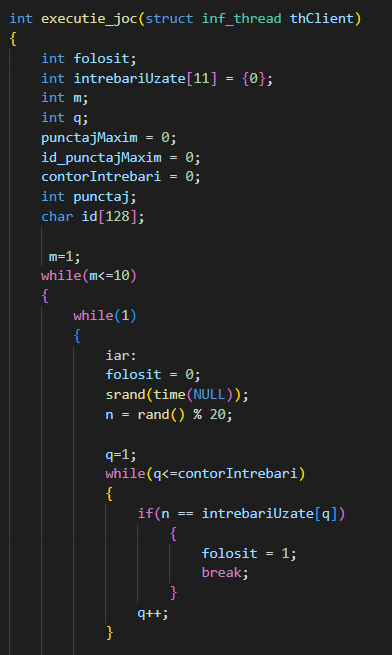
\includegraphics[scale=0.5]{server4}
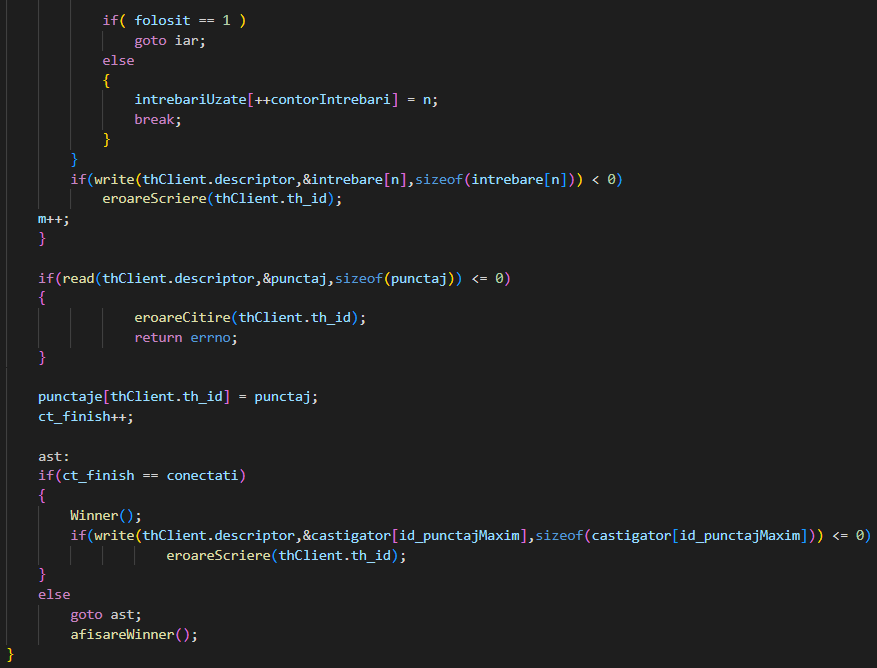
\includegraphics[scale=0.5]{server5}

\vspace{0.3cm}

\section*{Concluzii:}

$\quad$Serverul prelucreaza toate datele din baza de date si cele primite de la client, iar in client doar se afiseaza datele primite de la server, trimite inapoi raspunsurile si calculeaza punctele fiecarui client. Pe viitor as dori sa implementez functii care sa permita adaugarea de intrebari direct din server si alta care sa permita inregistrarea si clientilor care nu au conturi memorate in baza de date.

\section*{Bibliografie:}
$\quad$

1) \href{https://profs.info.uaic.ro/~computernetworks}{https://profs.info.uaic.ro/~computernetworks}

2) \href{http://zetcode.com/db/sqlitec/}{http://zetcode.com/db/sqlitec/}

3) \href{https://www.quora.com/How-do-I-put-a-time-limit-to-the-scanf-function}https://www.quora.com/How-do-I-put-a-time-limit-to-the-scanf-function{}

\end{document}


